\documentclass[12pt]{article}
\usepackage[spanish, es-tabla]{babel}
\usepackage{amssymb, amsmath}
\usepackage{float}
\usepackage{graphicx}
\usepackage[export]{adjustbox}
\title{Matemáticas para las Ciencias Aplicadas \\ Tarea 1}
\date{}
\author{Garcia Islas Fernando \\ Leo\\Mariana}
\begin{document}
\maketitle

\noindent {\large \bf3. Series de potencias}\\

    {\bf Definición 1} \textit{Una serie de potencias en $q$ es una suma infinita de la forma:}\[\sum_{k=1}^{\infty} a_k q^k \tag{3}\]

    \textit{donde $q$ es un número real cualquiera y $a_k$ para $k = 1, 2, 3, \dots$ son coeficientes en $\mathbb{R}$. Se dice que la serie (3) converge a un valor $S \in \mathbb{R}$, si}\[S = \lim_{n \to \infty} \sum_{k=1}^{n} a_k q^k \tag{4}\]


    \textit{es decir, que basta tomar un valor de $n$ suficientemente grande para que $S_n$, la suma finita o suma parcial desde 1 hasta $n$, se acerque a $S$ tanto como se quiera.}

    \textit{Si $a_k = 1$ para toda $k$, la serie de potencias}
    \[\sum_{k=1}^{\infty} q^k \tag{5}\]
    \textit{se llama serie geométrica de razón $q$.}


    En clase se demostró la siguiente fórmula cerrada para las sumas parciales de la serie (5):

    \[S_n = \sum_{k=1}^{n} q^k = \frac{q (1 - q^n)}{1 - q} \tag{6}\]

    y, con base en (6), se resolvió la paradoja de Zenón relativa al viajero que va de Atenas a Esparta. De hecho, se explicó por qué:

    \[\sum_{k=1}^{\infty} \frac{1}{2^k} = 1.\]

    \begin{enumerate}
    
%Punto 1 del ejercicio 3
        \item Recupere los argumentos vertidos en clase para explicar por qué, si $q \geq 1$, la serie (5) no converge o, dicho de otro modo, diverge a $+\infty$.\\
            Para $q>1$ los términos $q^k$ crecen sin limite a medida que k aumenta.En este caso, la serie diverge porque los términos no se acercan a cero ni a ningún número en especifico y la suma es infinita.\\
Es decir, para $q>1$ tenemos que $q^k \rightarrow \infty$ cuando $k\rightarrow \infty$ por lo que $S_n = \sum_{k=1}^{n} q^k \rightarrow \infty$
    

%Punto 2 del ejercicio 3
        \item Suponga ahora que $q \leq 0$. ¿Para qué valores de $q$ converge la serie (5)? En su respuesta, considere los siguientes casos:(a) $-1 < q \leq 0$, (b) $q = -1$ y (c)$q < -1$. Para tener una idea, es conveniente experimentar numéricamente en una hoja de cálculo (como se hizo en clase) con distintos valores de $q$ y, luego, buscar un argumento que explique el comportamiento general.\\
     \\ Para analizar mejor la serie obtendremos la formula de la suma infinita de la serie para apoyarnos a calcular cuando converge \\ 
    Escribimos la serie 
    \begin{eqnarray*}
        S=  q + q^2 + q^3+ q^4+ q^5+ ...
    \end{eqnarray*}
    
    Y multiplicamos cada termino de la serie por q
    \begin{eqnarray*}
           q S= q^2 + q^3+ q^4+ q^5+ q^6 ...
    \end{eqnarray*}
    Restamos la serie multiplicada de la original\\
    \begin{eqnarray*}
   S- qS =  (q + q^2 + q^3+ q^4+ q^5+ ...)& -  (q^2 + q^3+ q^4+ q^5+ q^6 ...)   \\
         S- qS= q \\
       S(1-q)=q \\
       S= \frac{q}{1-q}         
    \end{eqnarray*}\\

Así obtenemos la formula para obtener para las suma infinita de la serie.\\
 Observando la serie vemos que si $|q|<1$ va a converger y va a converger a la suma calculada anteriormente, ya que los  términos $q^k$  se acercan a cero conforme a k aumenta.\\
Observemos este caso y los otros dos:

\begin{itemize}
    \item $-1< q \leq 0$ \\
    Realizamos una tabla para analizar como se comporta la suma cuando q se encuentra en este rango:\\
          \begin{table} [H]
            \begin{center}
                \begin{tabular}{| c | c | c |}\\ \hline
                    q &     Serie & Suma de la serie  \\ \hline
                    -0.999 &  $(-.999)^1 + (-.999)^2 + (-.999)^3 +\ldots+(-.999)^n$ &  -0.4997   \\ \hline
                    -0.99 &  $(-.99)^1 + (-.99)^2 + (-.99)^3 +\ldots+(-.99)^n$ &    -0.4974\\ \hline
                    -0.9& $(-.9)^1 + (-.9)^2 + (-.9)^3 +\ldots+(-.9)^n$ &  -0.4736    \\ \hline
                    -0.1 & $(-.1)^1 + (-.1)^2 + (-.1)^3 +\ldots+(-.1)^n$  &  -0.0909  \\ \hline
                    -0.01& $(-.01)^1 + (-.01)^2 + (-.01)^3 +\ldots+(-.01)^n$ &   -0.0099 \\ \hline
                    -0.001& $(-.001)^1 + (-.001)^2 + (-.001)^3 +\ldots+(-.001)^n$ &   -0.0009  \\ \hline
                    -0.0001 & $(-.0001)^1 + (-.0001)^2 + (-.0001)^3 +\ldots+(-.0001)^n$ &  -0.00009   \\ \hline
                    0 & $(0)^1 + (0)^2 + (0)^3 +\ldots+(0)^n$& 0    \\ \hline
                \end{tabular}

                \label{tab:datos}
            \end{center}
          \end{table}
Observamos que en cada valor dentro del rango $-1<q\leq 0$ conforme k aumenta el valor de $q^k$ se acerca más a cero y la serie converge.

    
    


    
    \item $q=-1$\\
    En la tabla observamos como se comporta la serie con q=1, es decir como se comporta $\sum_{k=1}^{n} (-1)^k $
    \begin{table} [H]
    \centering
\begin{tabular}{| c | c | c |}
\hline
q &     Serie & Suma de la serie  \\ \hline
 -1 & $(-1)^1 + (-1)^2 + (-1)^3 +\ldots+(-1)^n$ = $-1+1-1+1-1+1...$ & Oscila entre 0 y -1  \\ \hline
\end{tabular}
\label{tab:datos}
\end{table}
La serie en este caso se convierte en una serie alternante que no converge. No converge a un limite finito, porque los términos no se estabilizan en torno a un valor único. En cambio la suma oscila entre 0 y -1.


    \item $q<-1$
\\
Para este caso tomamos diferentes valores negativos de q para observar el comportamiento de la serie:
   \begin{table} [H]
    \centering   
\begin{tabular}{| c | c | c |}
\hline
q &     Serie & Suma de la serie  \\ \hline
-2 &  $(-2)^1 + (-2)^2 +\ldots+(-2)^n$= $(-2) +4 + (-8) +(16)+ ...$ & \\ 
 -3 &  $(-3)^1 + (-3)^2 +\ldots+(-3)^n$=    $(-3) +9 + (-27) +(81)+ ...$ &\\ 
 -4& $(-4)^1 + (-4)^2 +\ldots+(-4)^n =(-4) +16 + (-64) +(256)+ ...$  &  No tienen     \\
 -5 & $(-5)^1 + (-5)^2 +\ldots+(-5)^n$ = $(-5) +25 + (-125) +(625)+ ...$ &  suma finita   \\ 
-10 &$(-10)^1 + (-10)^2 +\ldots+(-10)^n$ =$(-10) +100 + (-1000)+ ...$  &    \\ \hline
\end{tabular}

\label{tab:datos}

\end{table}
Observamos que cuando $q<-1$ la serie $\sum_{k=1}^{n} (q)^k $ diverge. Los términos de la serie alternan el signo y crecen en magnitud, lo que significa que no se acercan a ningún valor en especifico y la serie no tiene una suma finita.
    
\end{itemize}
\end{enumerate}


\noindent {\large \bf 4. Un balón de futbol americano} \\


 En este ejercicio se trata de calcular aproximadamente el volumen \( V \) de un balón de fútbol americano profesional suponiendo que su superficie se genera rotando, alrededor del eje horizontal, una curva \( y = y(x) \) que satisface que la longitud del eje entre las dos puntas del balón es de 28 cm y la circunferencia de la máxima sección circular transversal al eje mide 53 cm (véase la siguiente figura).\\
    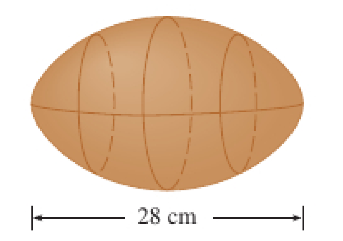
\includegraphics[width=0.5\textwidth, center]{balon.png}


Rebane la mitad derecha del balón en 10 cilindros de grosor \( \Delta x = 1.4 \) cm, de manera que las rebanadas intersecten el eje \( x \) en los valores de la siguiente partición del intervalo \([0, 14]\):

\[
P = \{x_k \mid x_k = k \Delta x \text{ para } k = 0, \ldots, 10\}
\]

es decir que:

\[
x_0 = 0, \quad x_1 = 1.4, \quad x_2 = 2.8, \quad x_3 = 4.2, \quad \ldots, \quad x_9 = 12.6, \quad x_{10} = 14.
\]

Entonces, si \( V_k \) es el volumen del \( k \)-ésimo cilindro,

\[
V \approx \sum_{k=1}^{10} V_k
\]
\renewcommand{\theenumi}{\alph{enumi}}
\begin{enumerate}
\item Suponga que la curva \( y = y(x) \) es un arco de parábola cuyo vértice coincide con el punto más alto de la máxima sección transversal perpendicular al eje \( x \) y que intersecta al eje horizontal en los puntos \((-14, 0)\) y \((14, 0)\). Entonces:
\renewcommand{\theenumi}{\arabic{enumi}}
\begin{enumerate}
    \item Muestre que la parábola es, aproximadamente, la gráfica de la función

\[
y(x) = -0.043 x^2 + 8.4352
\]

definida para \(-14 \leq x \leq 14\).\\
{\bf R:} Se tiene que la función de una parábola está denotada por:

\[ y(x)=ax^2+bx+c\]

Sabemos que la punto del vértice de la parábola con respecto al origen es $(0, \frac{53}{2\pi)}$ ya que la circunferencia del circulo situado a la mitad del  balón es 53 que se obtiene de la formula de  $P = 2\pi r$. Si sustituimos este valor en la fórmula de la parábola obtenemos $c$:

        \begin{align*}
            y(0)= \frac{53}{2\pi} &= a(0)^2+b(0)+c\\
            \frac{53}{2\pi} &= c
        \end{align*}
  
        Si ahora usamos los puntos donde la parábola toca al eje $x$ tendríamos a $a$ y $b$:
        
       \begin{align*}
            y(14)=0&= a(14)^2+b(14)+c &\quad y(-14)=0&= a(-14)^2+b(14)+c\\
             &= a(14)^2+b(14)+c &\quad &= a(-14)^2+b(-14)+c\\
            &= 196a+14b+c &\quad &= 196a-14b+c\\ 
        \end{align*}
            Si sumamos ambos resultados tenemos:\\
            
            \[
            \begin{array}{c}
            196a+14b+c\\
            196a-14b+c\\
            \hline
            392a +2c = 0\\
            \end{array}
            \]
        
        Si despejamos a $a$.
            
        \[a=- \frac{c}{196}\]
        Si queremos obtener a $b$, solo haría falta cambiar los signos a un valor y volverlos a sumar, y después despejar a $b$
        \[
        \begin{array}{c}
            196a+14b+c \\
            -196a+14b-c\\\hline
            28b = 0\\
            b=0
        \end{array}
        \]
    Teniendo ya las literales solo hace falta sustituirlas y desarrollar la ecuación:
\begin{align*}
   y(x)&=- \frac{\frac{53}{2\pi}}{196}x^2+\frac{53}{2\pi}\\ 
   y(x)&=- \frac{53}{392\pi}x^2+8.4352\\
   y(x)&=- -0.043 x^2+8.4352\\
\end{align*}



\item Muestre que la aproximación del volumen con los 10 cilindros circunscritos de grosor \( \Delta x = 1.4 \) cm y radios \( y(x_k) \) cm para \( k = 0, 1, 2, \ldots, 9 \) es:

\[
V \approx 2 \times 1825.5143 = 3651.0286 \text{ cm}^3
\]

{\bf R:} Con la función de la parábola para obtener los radios, generamos la siguiente tabla con los valores de los volúmenes:
\begin{table}[H]
    \centering
\begin{tabular}{|c|c|c|}\hline
    $V_k$ &Radio[cm] & Volumen[cm$^3$]\\\hline
     0 & 8.4352 & 312.9463 \\
     1 & 8.3508 & 306.7187 \\
     2 & 8.0978 & 288.4113\\
     3 & 7.676 & 259.1508\\
     4 & 7.0855 & 220.8149\\
     5 & 6.3264 & 176.0323\\
     6 & 5.3985 & 128.1828\\
     7 & 4.3019 & 81.3973\\
     8 & 3.0266 & 40.5578\\
     9 & 1.6026 & 11.2973\\\hline
      \multicolumn{1}{|c|}{}&Sumatoria & 1825.51 cm$^3$\\\hline
\end{tabular}
\label{tab:CilCirPar}
\end{table}
Si multiplicamos la sumatoria por dos obtenemos un resultado de 3651.02, valor aproximado al propuesto anteriormente.
\item Muestre que la aproximación del volumen con los 10 cilindros inscritos de grosor \( \Delta x = 1.4 \) cm y radios \( y(x_k) \) cm para \( k = 1, 2, \ldots, 10 \) es:
\end{enumerate}
\renewcommand{\theenumi}{\alph{enumi}}
\[
V \approx 2 \times 1512.5672 = 3025.1344 \text{ cm}^3
\]
{\bf R:} Así mismo como con los circunscritos, generamos otra tabla para los inscritos:

  
  
 \begin{table}[H]
    \centering
\begin{tabular}{|c|c|c|}\hline
    $V_k$ &Radio[cm] & Volumen[cm$^3$]\\\hline
     1 & 8.4352 & 306.7187 \\
     2 & 8.3508 & 288.4113 \\
     3 & 8.0978 & 259.1508\\
     4 & 7.676 & 220.8149\\
     5 & 7.0855 & 176.0323\\
     6 & 6.3264 & 128.1828\\
     7 & 5.3985 & 81.3973\\
     8 & 4.3019 & 40.5578\\
     9 & 3.0266 & 11.2973\\
     10 & 1.6026 & 0\\\hline
      \multicolumn{1}{|c|}{}&Sumatoria & 1512.5636 cm$^3$\\\hline
\end{tabular}
\label{tab:CilCirPar}
\end{table} 
  
 Y si lo multiplicamos por dos obtenemos 3025.1273, un valor aproximado al indicado.
  
 
\item Suponga ahora que la curva \( y = y(x) \) es la mitad superior de una elipse con centro en el origen, semieje horizontal \( a = 14 \) cm (sobre el eje \( x \)) y semieje vertical \( b = \frac{53}{2\pi} \approx 8.4352 \) cm (sobre el eje \( y \)).

\item Muestre que el arco de elipse es, aproximadamente, la gráfica de la función

\[
y(x) = 0.6025 \sqrt{196 - x^2}
\]

definida para \(-14 \leq x \leq 14\).

{\bf R:} Teniendo a $r_0 = \frac{53}{2\pi}$, como radio del circulo a la mitad del balón y semieje vertical b, y la función de una elipse como
\[\frac{x^2}{14^2}+\frac{y^2}{r_0^2}=1\]
se puede desarrollar para despejar $y$.
    \begin{align*}
        \left( \frac{x^2}{14^2} + \frac{y^2}{r_0^2} \right) \times 14^2r_0^2 &= 1 \times 14^2r_0^2\\
        x^2 r_0^2 + y^2 14^2 &= 14^2 r_0^2\\
        y^2 14^2 &= 14^2 r_0^2 - x^2 r_0^2\\
        y^2 &= \frac{14^2 r_0^2 - x^2 r_0 ^2}{14^2}\\
        y &=\sqrt{\frac{14^2r_0^2 -x^2r_0 ^2}{14^2}}\\
        y &=\frac{\sqrt{14^2r_0^2 -x^2r_0 ^2}}{14}\\
        y &=\frac{\sqrt{r_0^2(14^2 -x^2)}}{14}\\
        y &=\frac{r_0}{14}\left(\sqrt{14^2 -x^2}\right)\\
        y &=\frac{\frac{53}{2\pi}}{14}\left(\sqrt{196 -x^2}\right)\\
        y(x)=y &=0.6025\sqrt{196 -x^2}\\
    \end{align*}

\item Muestre que la aproximación del volumen con los 10 cilindros circunscritos de grosor \( \Delta x = 1.4 \) cm y radios \( y(x_k) \) cm para \( k = 0, 1, 2, \ldots, 9 \) es:

\[
V \approx 2 \times 2237.4593 = 4474.9186 \text{ cm}^3
\]
{\bf R:} Teniendo la función de los radios se genera la siguiente tabla para los volúmenes circunscritos:
  
     \begin{table}[H]
          \centering
            \begin{tabular}{|c|c|c|}\hline
                $V_k$ &Radio[cm] & Volumen[cm$^3$]\\\hline
                0 & 8.4352 & 312.9463\\
                1 & 8.3929 & 309.8169\\
                2 & 8.2647 & 300.4285\\
                3 & 8.0466& 284.7811\\
                4 & 7.7309 & 262.8749\\
                5 & 7.3051 & 234.7097\\
                6 & 6.7481 & 200.2856\\
                7 & 6.0239 & 159.6026\\
                8 & 5.0611 & 112.6606\\
                9 & 3.6782 & 59.4598\\\hline
                \multicolumn{1}{|c|}{}&Sumatoria & 2237.5665 cm$^3$\\\hline
            \end{tabular}
        \label{tab:CilCirPar}
    \end{table} 
    
Y multiplicando la sumatoria por 2 obtenemos 4475.1330, un valor aproximado al indicado.
\item Muestre que la aproximación del volumen con los 10 cilindros inscritos de grosor \( \Delta x = 1.4 \) cm y radios \( y(x_k) \) cm para \( k = 1, 2, \ldots, 10 \) es:

\[
V \approx 2 \times 1924.5279 = 3849.0558 \text{ cm}^3
\]
{\bf R:} Para los volúmenes inscritos se tiene la siguiente tabla:
  
     \begin{table}[H]
          \centering
            \begin{tabular}{|c|c|c|}\hline
                $V_k$ &Radio[cm] & Volumen[cm$^3$]\\\hline
                1 & 8.4352 & 309.8169\\
                2 & 8.3929 & 300.4285\\
                3 & 8.2647 & 284.7811\\
                4 & 8.0466 & 262.8749\\
                5 & 7.7309 & 234.7097\\
                6 & 7.3051 & 200.2856\\
                7 & 6.7481 & 159.6026\\
                8 & 6.0239 & 112.6606\\
                9 & 5.0611 & 59.4598\\
                10 & 3.6782 & 0\\\hline
                \multicolumn{1}{|c|}{}&Sumatoria & 1924.6201 cm$^3$\\\hline
            \end{tabular}
        \label{tab:CilCirPar}
    \end{table} 
    
Y multiplicando la sumatoria por 2 obtenemos 3849.2402, un valor aproximado al indicado.
    \end{enumerate}
    \noindent {\large \bf 8. Un jugador de béisbol} \\
    Un jugador de béisbol batea la pelota a 3 ft de altura sobre el plato en dirección a la barda del jardín central que está a 400 ft de distancia de home y tiene 10 ft de altura. La pelota sale con rapidez de 115 $\frac{ft}{s}$ y un ángulo de elevación de 50$^{\circ}$ sobre la horizontal.

\begin{enumerate}
    \item Reconstruya el argumento dado en clase para mostrar que el batazo es un home run. En particular, explique por qué:
    \begin{enumerate}
        \item La rapidez inicial de la pelota en la dirección horizontal es \( v_{0x} = 115 \cos (50^\circ) \), de manera que \( x = x(t) \), la posición horizontal de la pelota \( t \) segundos después del batazo es:
        \[
        x(t) = 73.9206 \ t. \tag{11}
        \]
        
        \item La rapidez inicial en la dirección vertical es \( v_{0y} = 115 \sin (50^\circ) \), lo que implica que \( y = y(t) \), la altura sobre el terreno de juego es (recuerde que, en el sistema inglés, la aceleración de la gravedad es \( g = 32 \ \text{ft/s}^2 \)):
        \[
        y(t) = 3 + 88.0951 \ t - 16 \ t^2. \tag{12}
        \]
        
        \item A partir de la fórmula (11), calcule el tiempo que tarda la pelota en estar a 400 ft de home y, con la fórmula (12), diga a qué altura estará la pelota justo en ese momento. ¿Su respuesta implica que la pelota superó la altura de la barda?
    \end{enumerate}
    
    \item En un tiro parabólico, la distancia horizontal entre el punto de partida y el lugar donde el móvil choca con algo se llama máximo alcance horizontal y se denota como \( x_{\text{max}} \). En este ejercicio, suponga que la pelota choca con un obstáculo que está a 5 ft de altura sobre el terreno de juego; muestre que:
    \[
    x_{\text{max}} \approx 405.3174 \ \text{ft}.
    \]
    
    \item A su vez, el máximo alcance vertical o altura máxima se denota como \( y_{\text{max}} \) y corresponde a la mayor distancia a la que llega el móvil en su desplazamiento hacia arriba y la alcanza en el momento en que la componente vertical de la velocidad vale cero; es decir, en el momento en el que la derivada de la posición vertical \( y = y(t) \) se anula. Con base en esto, muestre que:
    \[
    y_{\text{max}} \approx 124.2617 \ \text{ft}.
    \]
    
    \item Dibuje las gráficas de las funciones coordenadas \( x = x(t) \) y \( y = y(t) \) para \( 0 \leq t \leq t_{\text{imp}} \) donde \( t_{\text{imp}} \) es el tiempo en el que la pelota choca con el obstáculo que le impide seguir desplazándose parabólicamente.
    
    \item Dibuje la trayectoria de la pelota en el plano \( xy \).
\end{enumerate}
%Ejercicio 9

    \noindent {\large \bf 9. Una pista de carreras} \\
    Un arquitecto especializado en instalaciones deportivas quiere construir una pista de carreras de 1320 ft (un cuarto de milla) de largo alrededor de un campo de fútbol americano con la orientación que se muestra en la figura. El campo mide 360 ft de largo (incluyendo las zonas de anotación) y 160 \ \text{ft} de ancho. La pista consiste de dos semicírculos y dos segmentos rectilíneos cuya longitud mínima es la del largo del campo.

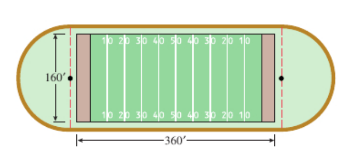
\includegraphics[width=0.5\textwidth, center]{cancha.png}

\begin{enumerate}
    \item Mostrar que es posible construir una pista de un cuarto de milla alrededor del campo de fútbol. (Se sugiere calcular la longitud de la pista más corta que podría construirse alrededor del campo).\\
        {\bf R:} Si calculamos la longitud mínima que podemos construir alrededor del campo y se la restamos a los 1320 ft que queremos tenemos que:
        \begin{align*}
        2(360)+2\pi 80 = 720 + 502.6548 = 1222.6548
        1320-1222.6548 = 97.3452
        \end{align*}
    Si esto lo dividimos entre 2 y se lo agregamos a la longitud de los laterales del campo y mantenemos la de los semicírculos, obtendríamos una pista de 1320 ft, con las siguientes dimensiones: lados rectos: 408.6726; semicírculos: 502.6548.
    
    \item Sea \( L \) la longitud, en pies, de una de las partes rectas de la pista y sea \( x \) la distancia, en pies, entre la línea lateral del campo y una de las partes rectas de la pista. Muestre que \( L \) como función de \( x \) viene dada por:
    \[
    L(x) = 660 - 80 \pi - \pi x
    \]
    
    {\bf R:} En base que la forma de crear la pista es sumar los lados rectos más los dos perímetros semicírculos (o una circunferencia de un círculo) se puede desarrollar la siguiente ecuación:
    
    \[
    2y+2\pi(80+x)=1320
    \]
    
    donde $y$ es la longitud del lado recto de la pista y $x$ es la distancia entre el largo de la campo y el lado recto de la pista.\\
    Si despejáramos $y$ tenemos:
    \[
    y=660-80\pi-\pi x
    \]
    
    y grafique esta regla de correspondencia para \( 0 \leq x \leq 20 \). 
    
    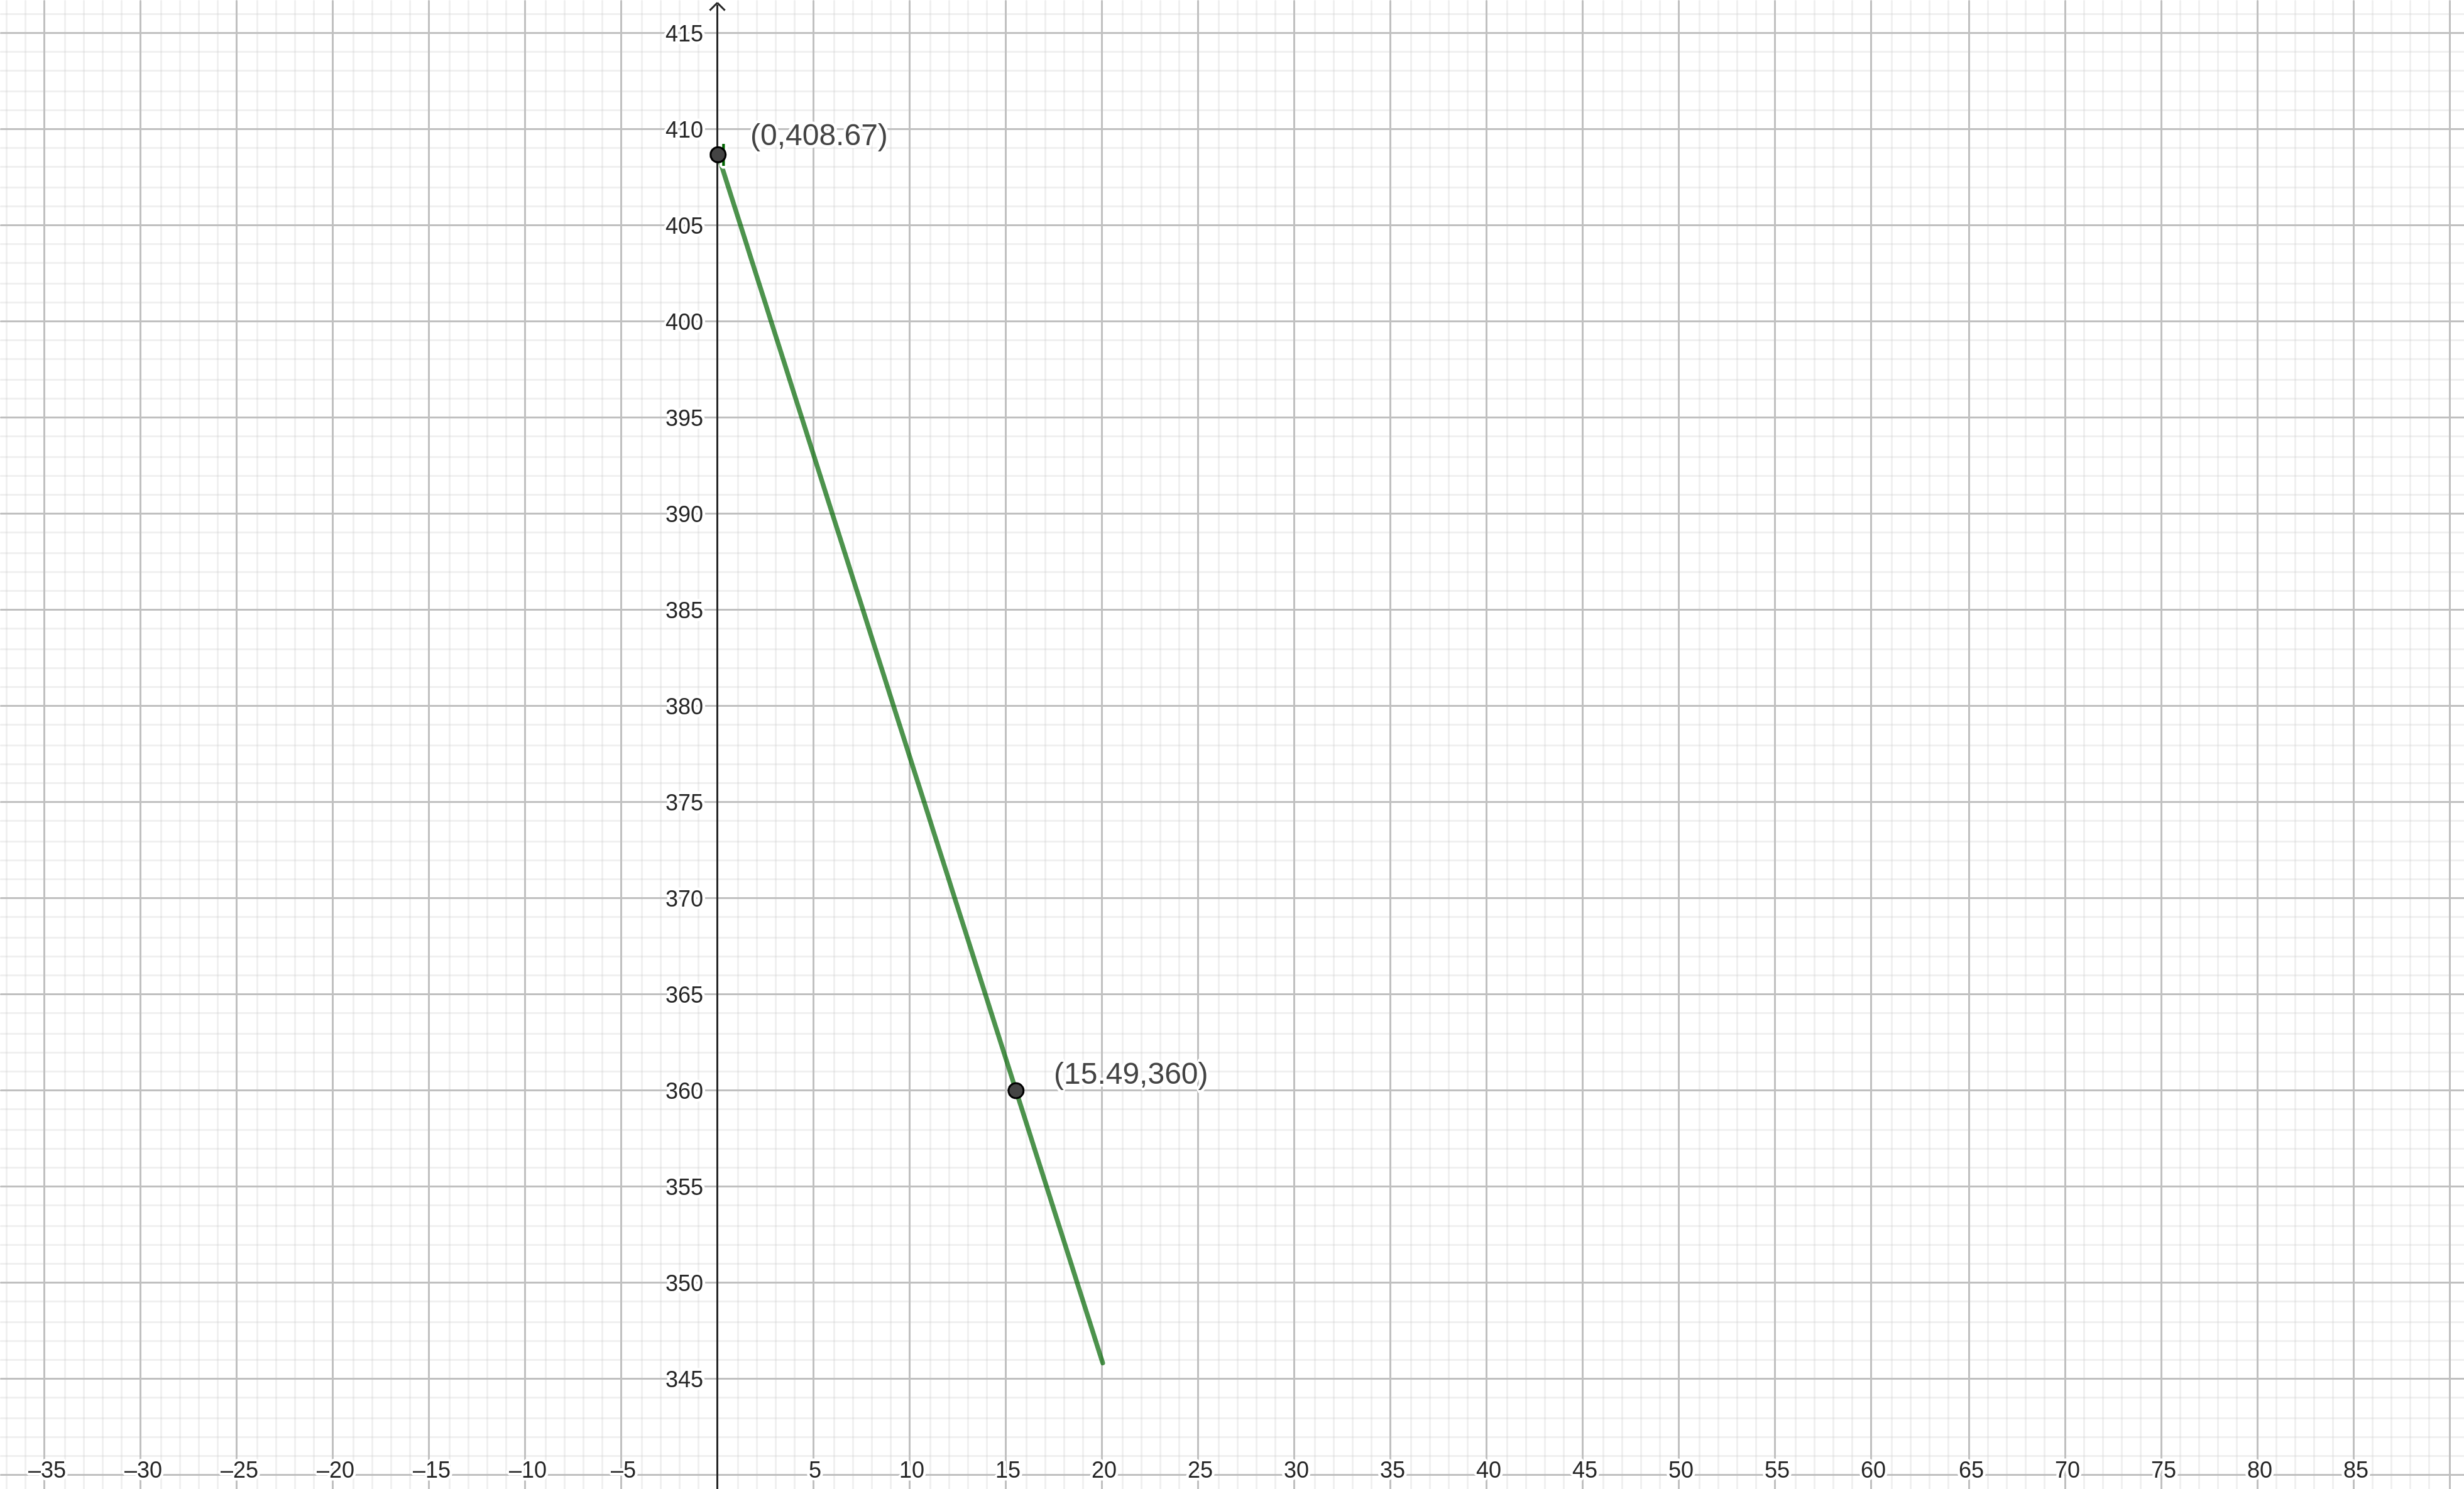
\includegraphics[width=0.7\textwidth, center]{graficapista.png}
     
    Con base en esta gráfica:
    \begin{enumerate}
        \item Estime la mínima longitud de la parte recta de la pista y, luego, muestre que el valor de \( x \) para el que esta ocurre es aproximadamente 15.49 ft.\\
        {\bf R:} Según la gráfica y la información del problema, la mínima longitud sería de 360, sustituyendo esto a la ecuación y despejando a x obtenemos:
        \begin{align*}
            360&=660-80\pi-\pi x\\
            360-600&=-80\pi-\pi x\\
            -300&=-80\pi-\pi x\\
            -300&=-\pi(80+x)\\
            \frac{-300}{-\pi}&=80+x\\
            95.4929 - 80 &= x\\
            x&=15.4929
        \end{align*}
        Por lo tanto, para la mínima longitud de la parte recta, el valor de $x$ es aproximadamente 15.4929.
        
        \item Estime la máxima longitud de la parte recta de la pista y, luego, muestre que el valor de \( L \) para el que esta ocurre es aproximadamente 408.67 \ \text{ft}.\\
    {\bf R:} Según la gráfica, la máxima longitud sería de 408.6725, sustituyendo esto a la ecuación y despejando a x obtenemos:
        \begin{align*}
            408.6725&=660-80\pi-\pi x\\
            408.6725-600&=-80\pi-\pi x\\
            -251.3275&=-80\pi-\pi x\\
            -251.3275&=-\pi(80+x)\\
            \frac{-251.3275}{-\pi}&=80+x\\
            80 - 80 &= x\\
            x&=0
        \end{align*}
    Por lo tanto, para la máxima longitud de la parte recta, el valor de $x$ es aproximadamente 0.
    \end{enumerate}
\end{enumerate}

    \noindent {\large \bf 11. Una caja con tapa superior} \\
    De un pedazo rectangular de cartón de 6 ft por 10 ft se va a fabricar una caja con tapa superior doblando a lo largo de las líneas punteadas, cortando cuatro cuadrados del mismo tamaño (véase la Figura 1) y plegando dentro de la caja las dos pestañas extras.

\begin{figure}[h]
    \centering
    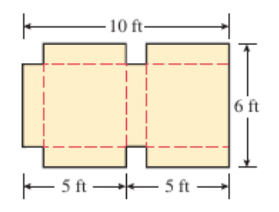
\includegraphics{caja.png}
    \caption{ Caja de 6 ft $\times$ 10 ft}
\end{figure}

\begin{enumerate}
    \item Hallar una fórmula que exprese el volumen \( V \) de la caja como función de la longitud \( x \) de los lados de los cuadrados que se cortan.\\
    
    \item 
    {\bf R:} Según la Figura 1, tenemos que un lado sera igual a $6-2x$, otro a $5-x$ y la altura igual a $x$, por consiguiente tenemos la siguente ecuación:
    \begin{align*}
    V&=x(5-x)(6-2x)\\
    V&=5x-x^2(6-2x)\\
    V&=30x-6x^2-10x^2+2x^3\\
    V&=2x^3-16x^2+30x
    \end{align*}
    
    \item Describa, mediante una desigualdad que acote los posibles valores de \( x \), el dominio de definición de la función \( V = V(x) \) del inciso anterior.\\
    
    
    {\bf R:} Ya que el valor de $x$ se le quitará como un cuadrado a ambos lados del cartón, entonces el máximo corte que se puede hacer es al lado más corto, siendo este menor a 3, ya que más de 3 reduciría los 6 ft. Así mismo tiene que ser mayor a 0, ya que si no quitamos nada no podríamos armar una caja. Entonces el dominio de $V=2x^3-16x^2+30x$ sería: $0<x<3$.
    
    \item Usar la gráfica de \( V = V(x) \) para dar valores aproximados de las dimensiones de la caja de máximo volumen.\\
    
    
    {\bf R:} Según la siguiente gráfica\\
    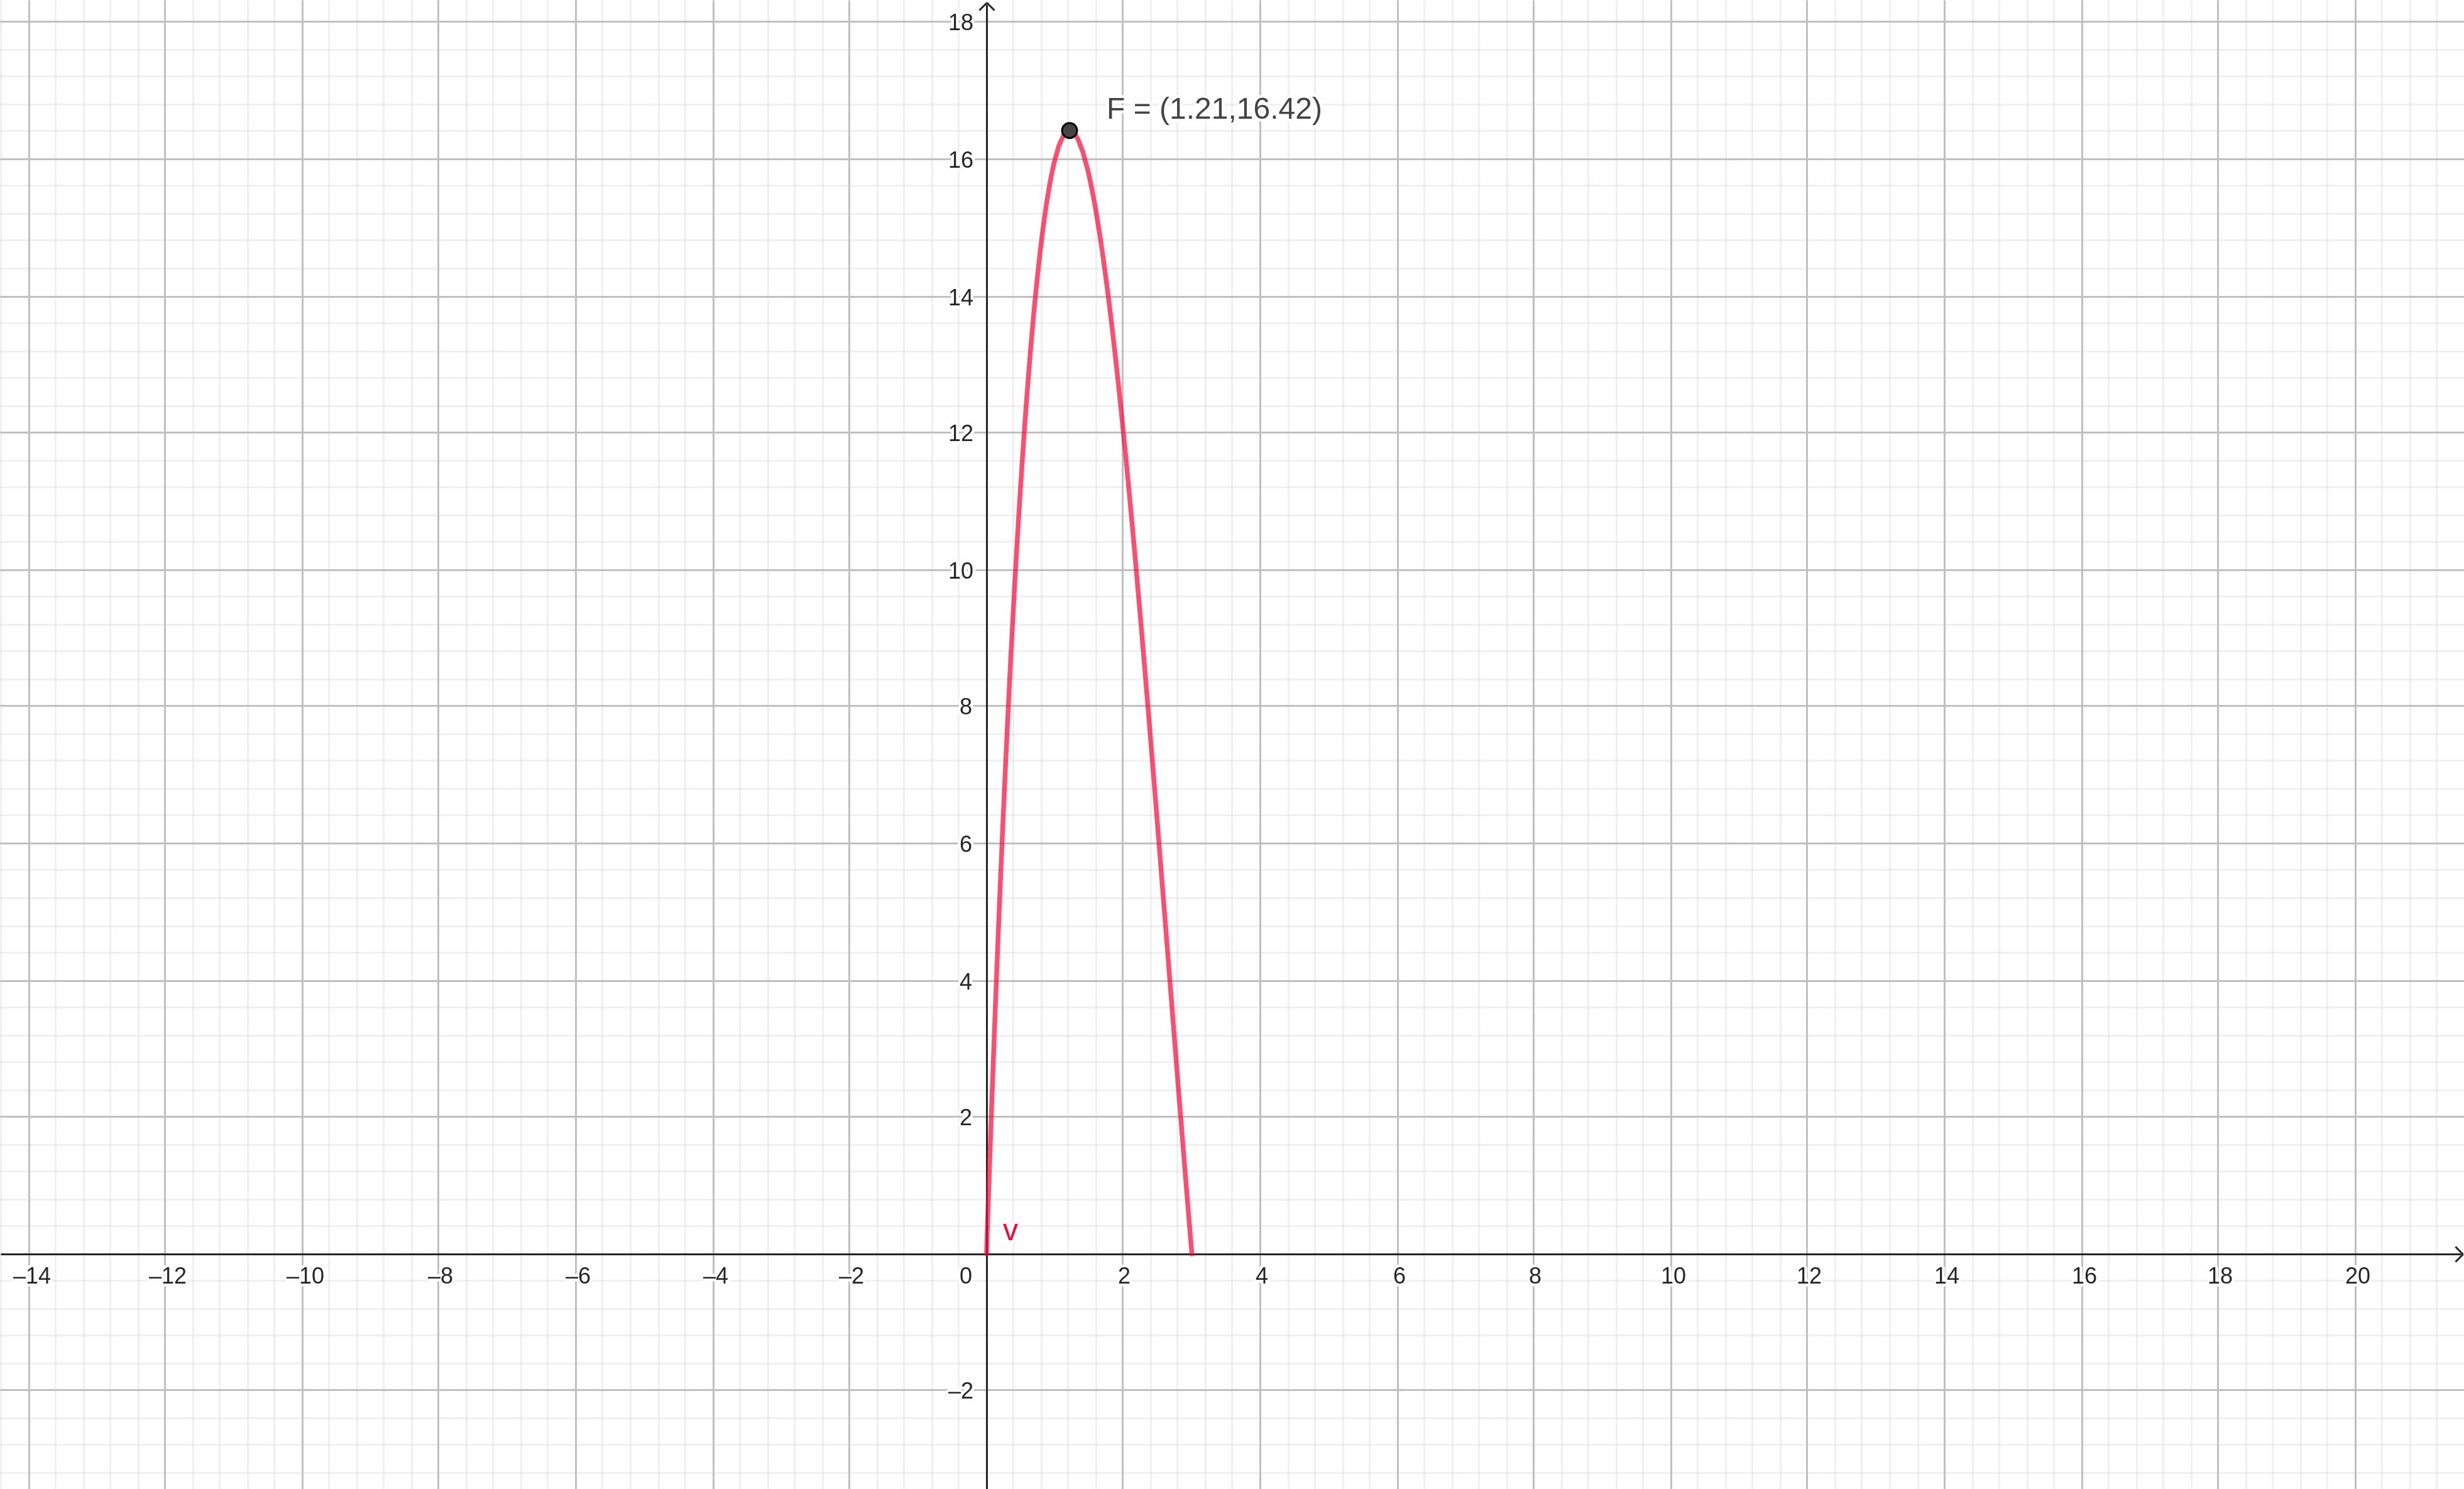
\includegraphics[width=0.7\textwidth, center]{graficacaja.png}
    el punto más alto, o el punto $x$ donde está el máximo volumen es 1.21, sustituyendo en la ecuación tenemos:
    \begin{align*}
    V&=2(1.21)^3-16(1.21)^2+30(1.21)\\
    V&=2(1.7715)-16(1.4641)+36.3\\
    V&=3.543-23.4256+36.3\\
    V&=-19.8826+36.3\\
    V&=16.4174
    \end{align*}
    Por lo tanto, el valor del volumen máximo es de 16.4174, con $x=1.21$
\end{enumerate}

    \noindent {\large \bf 13. Un hato de 20 borrejos cimarrones} \\
    Un hato de 20 borregos cimarrones se libera en un área protegida para la recuperación de la población silvestre de esa especie en peligro de extinción. Se espera que, con un manejo cuidadoso, la población de borregos \( N = N(t) \) después de \( t \) años sea

\[
N(t) = \frac{220}{1 + 10 e^{-0.1863 t}}
\]

y que la población será capaz de autosustentarse sin supervisión cuando llegue a 80 individuos.

\begin{enumerate}
    \item Dibuje la gráfica de \( N = N(t) \).\\
    {\bf R:}\\
    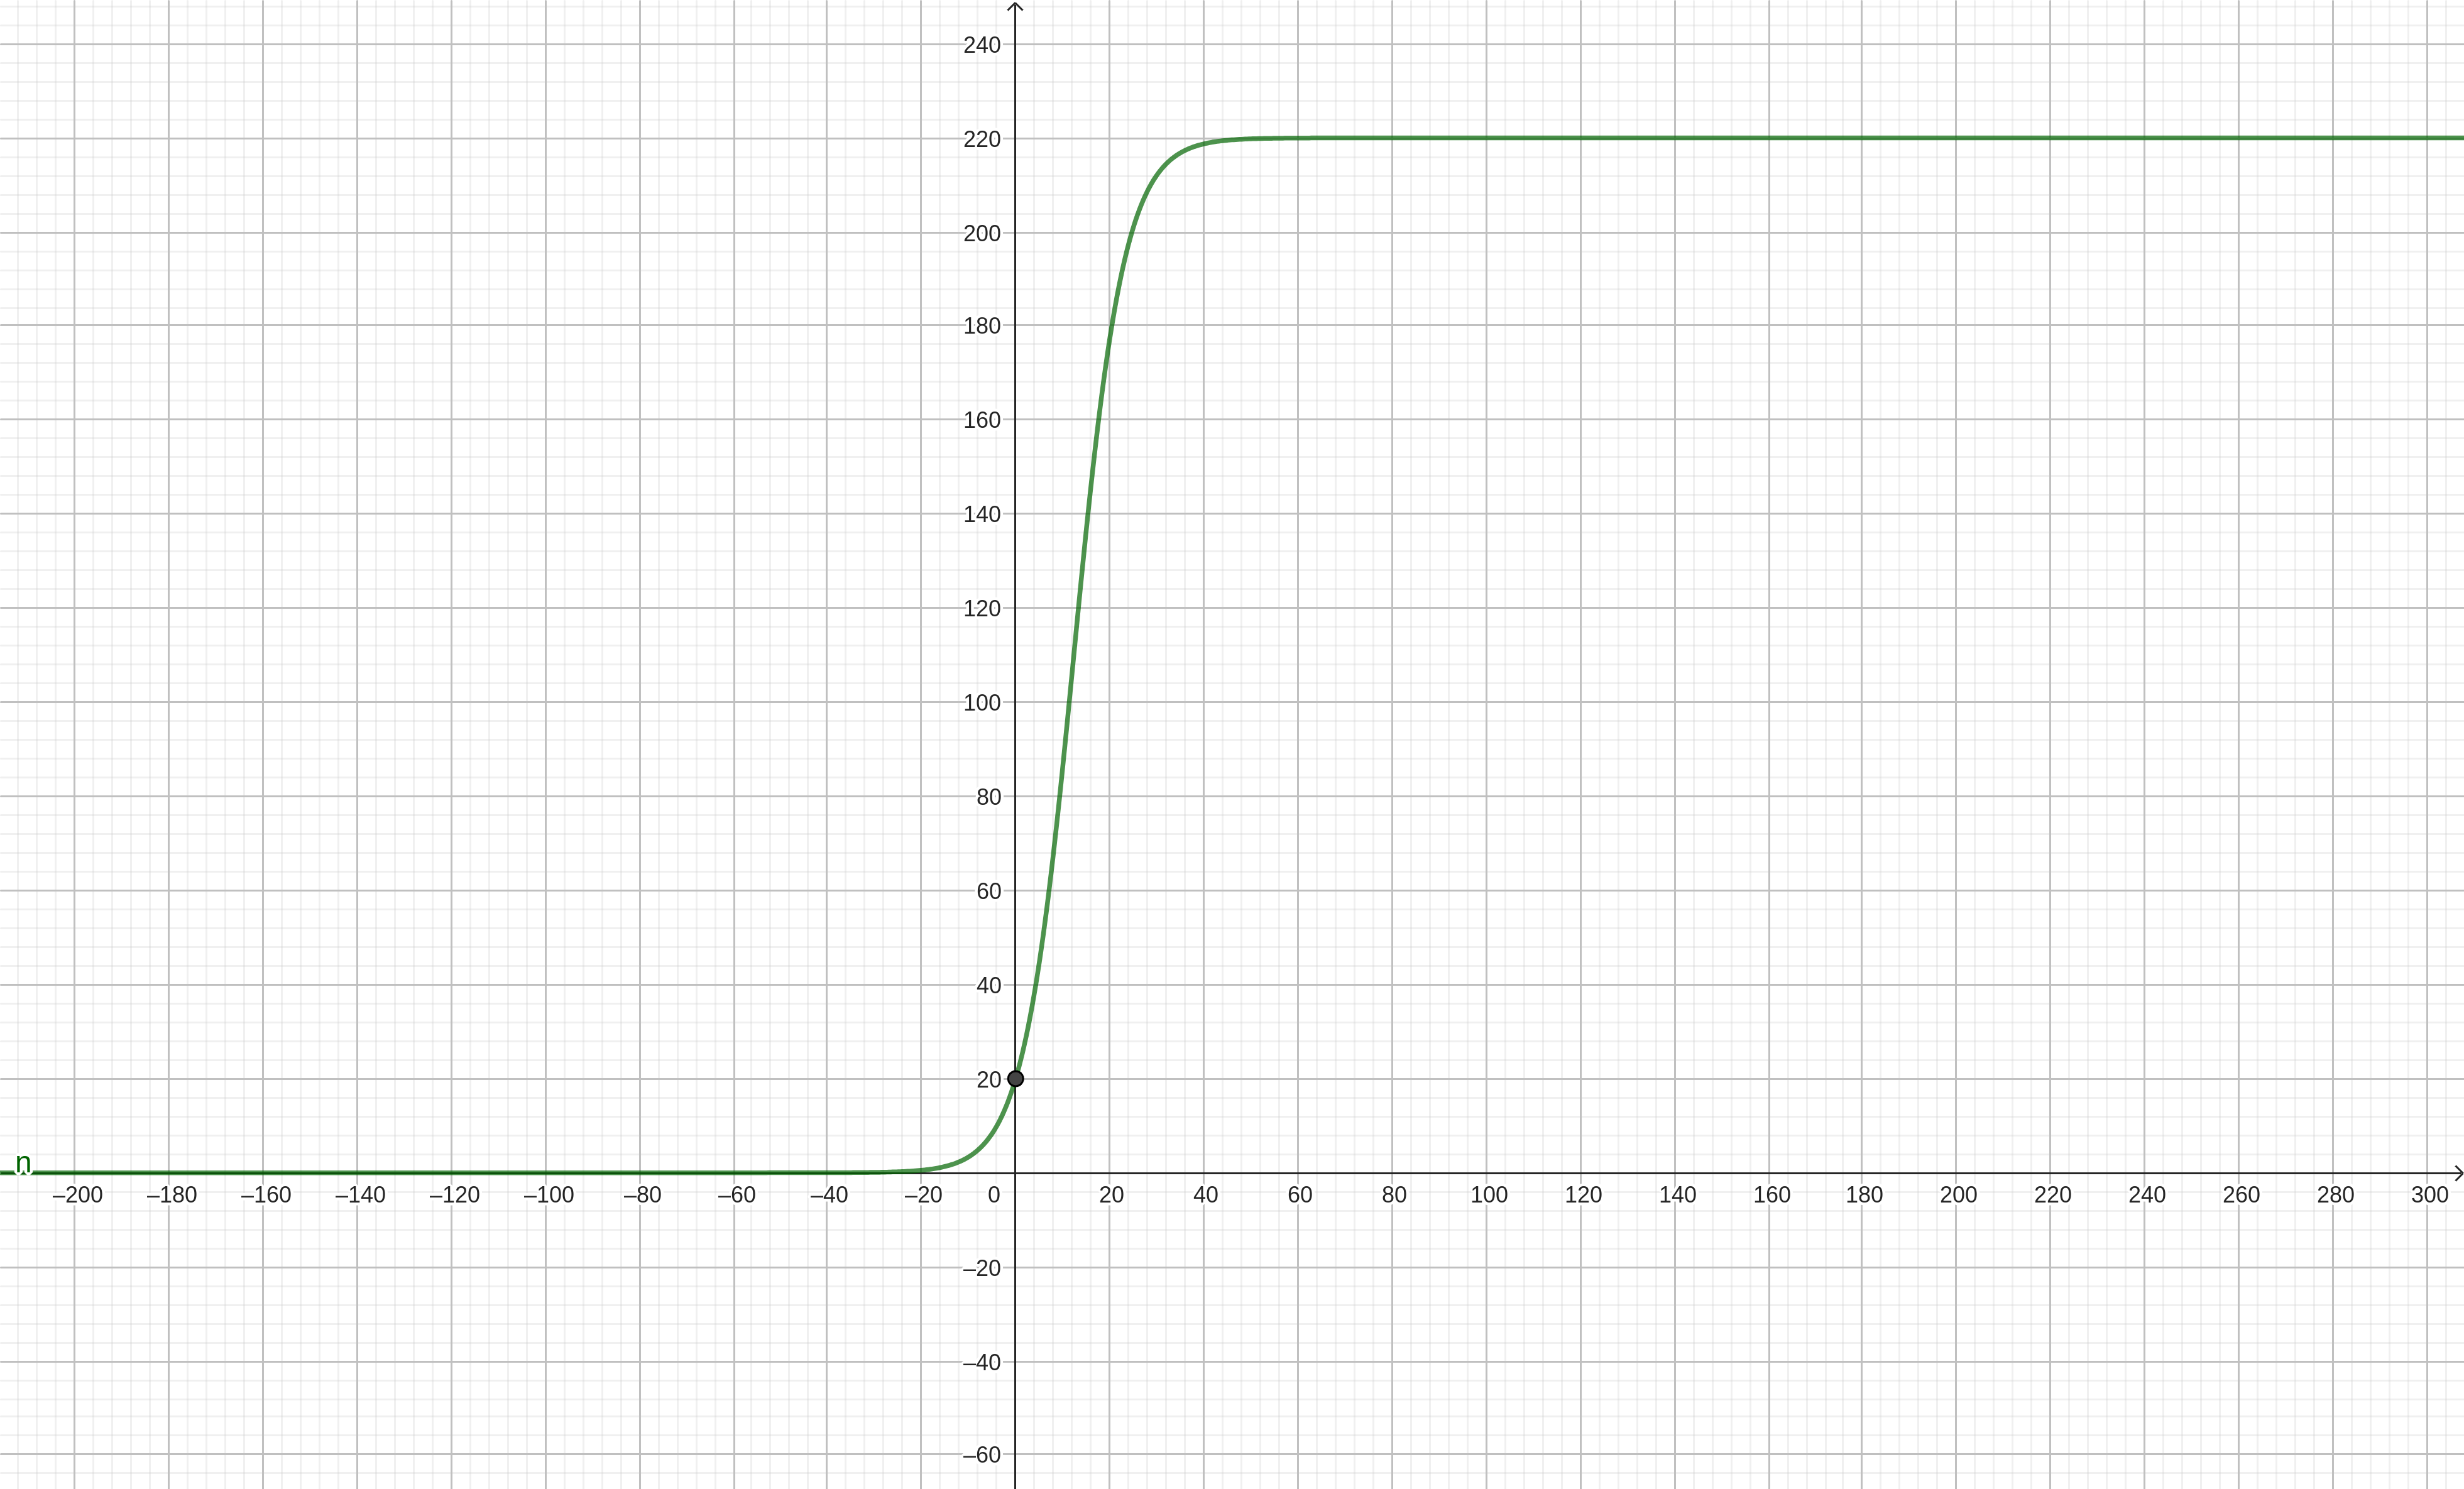
\includegraphics[width=1\textwidth, center]{graficaborregos.png}
    
    \item Muestre que el programa de repoblación deberá sostenerse por lo menos durante 9.36 años antes de que la población sea autosustentable.\\
    {\bf R:} Teniendo la función, sustituimos el valor de 80 y desarrollamos para despejar a $t$, que sería el tiempo que tardaría:\\
    \begin{align*}
        80 &= \frac{220}{1 + 10 e^{-0.1863 t}}\\
        1 + 10 e^{-0.1863 t}(80) &= 220 \\
        1 + 10 e^{-0.1863 t} &= \frac{220}{80} \\
        10 e^{-0.1863 t} &= 2.75 -1 \\
        e^{-0.1863 t} &= \frac{1.75}{10} \\
    \ln (e^{-0.1863 t}) &= \ln (0.175) \\
        -0.1863 t &= -1.7429\\
        t &= \frac{-1.7429}{-0.1863}\\
        t&=9.3553
    \end{align*}
    
    Obtuvimos un valor aproximado, lo cual nos confirma que habrá 80 borregos cimarrones en 9.36 años.
    
    \item Según este modelo, ¿cuántos borregos cimarrones podrían habitar el área protegida? Justifique su respuesta en términos de la gráfica de \( N = N(t) \) y confirme su respuesta calculando el límite \( \lim_{t \to \infty} N(t) \).
\end{enumerate}


    \noindent {\large \bf 14. Modelo para la variacion diurna} \\
    La Figura 3 muestra un modelo para la variación diurna (i.e., durante un período de 24 horas) de la altura y de la marea sobre el nivel medio del mar en una caleta de la bahía de San Francisco. Calcular los valores de \( y_0 \), la altura media; de la amplitud \( A \), la frecuencia angular \( \omega \) y la fase \( \phi \) de una función armónica para el modelo con regla de correspondencia:

\[
y(t) = y_0 + A \sin(\omega t + \phi),
\]

si se supone que \( t = 0 \) corresponde a la medianoche, el tiempo se mide en horas y la altura, en pies.

    
\end{document}
